\documentclass[letterpaper, 12pt]{article}
%%\documentclass[letterpaper, 11pt, twocolumn]{article}
\usepackage{url}
\usepackage{ctable}
\usepackage{overcite}
\usepackage{amsmath,amssymb}      % for \AA etc
\usepackage[onehalfspacing]{setspace}
\usepackage{graphicx}
\usepackage{fullpage, times}
\usepackage{algorithmic}
\usepackage{algorithm}
\usepackage{longtable}

\DeclareGraphicsExtensions{.pdf,.png}
\onehalfspacing

\bibliographystyle{jcics}

\usepackage{anysize}
%\marginsize{1in}{2in}{1in}{1in}
%\marginparwidth 1.75in
%\newcommand{\mnote}[1]{\marginpar{\raggedright{\footnotesize\textbf{#1}}}}

\def\imagetop#1{\vtop{\null\hbox{#1}}}

%%%
%%% Don't change the size of the figures as they are defined for
%%% a single column environment, which is what we will be submitting
%%% as
%%%

\begin{document}
\title{Exploring Uncharted Territories - Predicting Activty Cliffs in
  Structure-Activity Landscapes}
\author{Rajarshi Guha${}^{\ddagger}$\\
NIH Center for Advancing Translational Sciences \\ 9800 Medical Center Drive  Rockville, MD 20850}
\date{}

\maketitle
\begin{abstract}
  The notion of activity cliffs is an intuitive approach to characterizing structural features that
  play a key role in modulating biological activity of a molecule. A variety of methods have been
  described to quantitatively characterize activity cliffs, such as SALI and SARI. However, these
  methods are primarily retrospective in nature; highlighting cliffs that are already present in the
  dataset. The current study focuses on employing a pairwise characterization of a dataset to train
  a model to predict whether a new molecule will exhibit an activity cliff with one or more members
  of the dataset. The approach is based on predicting a value for pairs of objects rather than the
  individual objects themselves (and thus allows for robust models even for small structure-activity
  relationship datasets). We extracted structure-activity data for several ChEMBL assays and
  developed random forest models to predict SALI values, from pairwise combinations of molecular
  descriptors. The models exhibited reasonable RMSE's though, surprisingly, performance on the more
  significant cliffs tended to be better than on the lesser ones. Our results indicate that the
  predictive models are able to prioritize molecules in terms of their ability to activity cliffs
  and can be used as a way to extend an observed activity landscape to identify molecules that could
  lead to significant improvements in activity. Conversely, the method can be used to deprioritize
  molecules that are predicted to show an activity cliff with a potent molecule already in the
  dataset.
\end{abstract}

\section{Introduction}

The landscape paradigm for structure-activity relationship (SAR) data was first proposed 20 years
ago \cite{Johnson:1990ys} and has recently seen a resurgence with a number of studies describing new
ways to quantify and visualize activity landscapes. When SAR data is viewed as a landscape, with the
X-Y plane representing structural characteristics (which will usually be a 2-dimensional
representation of a multi-dimensional descriptor space) and the Z-axis representing the observed
activities, one can identify two broad types of regions on the landscape - smooth rolling regions,
corresponding to set of molecules exhibiting continuous SAR (i.e., similar structures and similar
activities) and rough, gorge-like regions (i.e., very similar structures, but large differences in
activity) corresponding to molecules that exhibit SAR discontinuity. The latter have also been term
activity cliffs \cite{Maggiora:2006aa}. From a medicinal chemistry point of view, the latter regions
of a landscape can be the most interesting as they can provide insight into structural features that
are key to improving (or conversely reducing) potency. There is a rich history of methods that have
correlated structural differences with corresponding differences in activity -- matched molecular
pairs \cite{Leach:2006aa}, SAS maps \cite{Maggiora:2011kx} and more recently SALI \cite{Guha:2008aa}
and SARI \cite{Peltason:2007aa}. Both SALI and SARI focus on numerically characterizing a structure
activity landscape. The former is defined for a pair of molecules as
\begin{equation}
  \label{eq:1}
  S_{i,j} = \frac{|A_i - A_j|}{1 - sim(i,j)}
\end{equation}
where $A_i$ and $A_j$ represent the observed activities of molecules $i$ and $j$, and $sim(i,j)$
represents the structural similarity between the two molecules (usually based on some form of
fingerprint similarity). Using the SALI metric, one can take a collection of $n$ molecules and
represent them as an $n \times n$ matrix of SALI values - larger values representing more
significant activity cliffs. The SARI approach is based on a score defined as
\begin{equation}
  \label{eq:2}
  \mathrm{SARI} = \frac{1}{2} \left(\mathrm{score}_{cont} + (1 -
    \mathrm{score}_{disc}) \right)
\end{equation}
where the individual score terms are derived on the basis of potency and pairwise similarities. The
reader is referred to Ref. \citen{Peltason:2007aa} for a detailed discussion of this approach.

In either case, one can take the numerical values and visualize them in a variety of ways ranging
from heatmaps of SALI matrices to network representations \cite{Wawer:2008aa,Guha:2008aa}. These
visualizations then allow the user to explore the landscape, quickly identifying a range of activity
cliffs, which an then be examined in detail. Apart from identifying individual activity cliffs, a
variety of other SAR constructs, such as ``activity ridges'' \cite{Vogt:2011bs} and multitarget
landscapes\cite{Dimova:2011fk} can also be identified and characterized.

A feature common to all, recently published work on activity landscapes is that they are primarily
retrospective. That is, the methodologies developed are used to analyze SAR datasets for which
activities have already been experimentally obtained. For example, using the SALI, one can
characterize SAR patterns in a dataset but does not provide insight into whether a new molecule may
be part of an activity cliff, with respect to the original dataset. A number of applications have
attempted to extract SAR rules based on the landscape (e.g., similarity potency trees
\cite{Wawer:2010fv} and multi-target landscape analyses \cite{Hu:2010kl}) or directly identify
structural modifications that lead to activity cliffs \cite{Wassermann:2010oq, Peltason:2009vn}.

\subsection{Motivation}
\label{sec:motivation}
The preceding discussion highlights the utility of retrospective analyses of SAR data using the
activity landscape paradigm. But equally, if not more, interesting is determining whether a new,
untested molecule might be an activity cliff in the context of the original dataset. For the
remainder of this work we focus on the use of SALI to quantify activity landscapes. More
specifically, the ability to \emph{predict} SALI values would be useful as it would allow us to both
fill in empty regions of an activity landscape as well as extend a structure-activity
landscape. Note that this approach to expanding the extent of a SAR dataset does not lend itself to
scaffold hopping since the premise of scaffold hopping is that one generates new cores, which differ
substantially from the starting structure.

In traditional QSAR modeling approaches, one simply predicts the activity of a new molecule and
would then evaluate the SALI (or SARI or some other measure) to determine whether the molecule leads
to an activity cliff. However, the fact that an activity cliff represents a SAR
discontinuity\cite{Maggiora:2006aa} implies that most statistical and machine learning methods will
be unlikely to predict very different activities for two structurally similar molecules. In other
words, a new molecule, similar to a subset of the training set, will tend to have a predicted value
that is similar to those molecules, rather than a drastically different value.

An alternative approach, that is the focus of this paper, is to directly predict SALI values for
pairs of molecules. Thus rather than predict individual activities, we predict SALI values for pairs
of molecules. This approach is somewhat similar to the SPREAD method \cite{Scheiber:2009fk} which
identified substructures that were predictive of activity differences. However, our solution
considers both activity differences and structural similarities. As a result, instead of ranking
compounds in terms of their predicted activity, we instead rank a compound in terms of its predicted
SALI; i.e., its predicted ability to exhibit an activity cliff when paired with other molecules in
the dataset. This approach could be useful when deciding how far to extend an analog series as well
as prioritizing scaffolds for further study.

This does not completely alleviate the problem of discontinuities, since SALI values are infinite
when the $T_c$ is 1.0.  However, predicting SALI values allows us to work with smaller datasets
(since the objects to predict are pairs of molecules), that would ordinarily lead to unreliable
models if we were working with activities. Of course, this means that the approach is not practical
for very large datasets.


The paper is organized as follows. Section \ref{sec:datasets} describes the datasets used in this
study. Section \ref{sec:methodology} presents the methodology we employ to predict activity cliffs
and Section \ref{sec:applications} discusses the results of the predictive models. Finally, Sections
\ref{sec:discussion} and \ref{sec:conclusions} discusses some of the issues underlying this approach
and possible extensions of this work.

\section{Datasets}            
\label{sec:datasets}
For this study we considered a number of datasets, which are summarized in Table \ref{tab:data}. The
Cavalli dataset was employed in our previous studies consisted of 30 molecules studied by Cavalli et
al\cite{Cavalli:2002aa} as possible hErg inhibitors using a CoMFA modeling approach. The reported
endpoint for the molecules was a pIC$_{50}$.The remaining datasets were obtained from ChEMBL. All
three assays involved direct binding to a human target and we considered the subset of molecules in
each assay that had non-censored experimental values. The Costanzo dataset\cite{Costanzo:2005uq}
consisted of 60 $\alpha$-ketoheterocyclic inhibitors of $\alpha$-thrombin. The reported
$\mathrm{IC_{50}}$ values ranged from 3 nM to 82 $\mu$M. The Kalla dataset\cite{Kalla:2006kx}
consisted of 38 8-(C-4-pyrazolyl) xanthines, identified as antagonists of the A2B adenosine
receptor. The reported $K_i$ values ranged from 0.9 nM to 42 $\mu$M. Finally, the Dai
dataset\cite{Dai:2007kl} consisted of 44 3-aminoindazole derivatives studied for their ability to
inhibit the VEGF and PDGF receptor families, with $\mathrm{IC_{50}}$ values ranging from 3 nM to
12~$\mu$M.

% To obtain the remaining datasets we mined the
% ChEMBL database to identify assays with the following constraints:
% cntaining between 30 and 500 molecules, direct binding to a human
% protein target, a data type of $K_i$ or $\mathrm{IC_{50}}$ and a
% reported confidence score of 8 or more. This identified 780
% assays. For each assay we considered those molecules with non-censored
% measured values and identified those assays for which at least one
% pair of molecules exhibited 1000-fold (or better) difference in
% activity. This led to a final set of 347 assays. From this set we
% considered three assays for three different targets

\section{Methodology}
\label{sec:methodology}
As noted above, the problem of identifying activity cliffs involving new molecules can be reduced to
predicting the SALI value for the new molecule and a preexisting molecule. Note that this does not
result in an activity prediction for the new molecule; rather, it allows us to rank a set of new
molecules in terms of their predicted ability to exhibit a significant activity difference with
respect to one or more of the molecules in the training set.

Given a training set of $N$ molecules, we generate a new training set of $\frac{N(N-1)}{2}$ objects,
where each object is a pair of molecules from the original training set. The dependent variable for
each pair $i,j$, is the SALI value, $S_{i,j}$. SALI values were evaluated using the 1051-bit BCI
keyed fingerprints (Digital Chemistry, UK) or the CDK\cite{Steinbeck:2006aa,Steinbeck:2003bh}
1024-bit path fingerprints. Based on the definition of SALI, it is possible that a pair of molecules
have a $T_c = 1.0$ resulting in infinite values. For such cases, we replaced the infinite value with
the highest non-infinite SALI value for that dataset.

The next step is to generate a set of independent variables. Since the new dataset consists of pairs
of molecules, we consider the descriptors for the resultant objects as a function of the descriptor
values of the individual molecules. For an object, representing the $i$'th and $j$'th molecules, its
descriptor vector can be taken as the arithmetic mean of the descriptor vectors of the individual
molecules. We denote this aggregation function as $f_{\textrm{mean}}$. Alternative functions that
were investigated included the absolute difference of the individual descriptors, denoted by
$f_{\textrm{diff}}$ and the geometric mean of the individual descriptor vectors, denoted by
$f_{\textrm{geom}}$.

Given the independent and dependent variables for the pairwise dataset, we can now proceed to model
development. For this study we focused on the use of random forest models\cite{Breiman:1984aa}. This
was motivated by the fact that such models tend not to overfit the training data (given a
sufficiently large number of trees) and the fact that the algorithm implicitly performs feature
selection. As a result, this allows us to forgo an explicit feature selection step and work directly
with the descriptor pool (after removal of correlated and constant descriptors). Furthermore, there
is no reason, \emph{a priori} to assume that the underlying SAR's are linear. A random forest model,
being an algorithmic approach\cite{Breiman:2001nx} (as opposed to a distributional one such as
linear regression) makes no such assumptions. We employed the implementation of random forest from
the \texttt{randomForest} package, in R 2.11.0\cite{r}. The models were built using 500 trees, and
randomly sampled the descriptor pool for a given dataset, using $\sqrt(N)$ descriptors at a time,
where $N$ is the number of descriptors in the pool. By default, the method builds individual trees
using 63\% of the dataset and tested on the remainder (the so called out-of-bag data). The final
predicted values for the entire dataset are obtained by averaging the predictions for each
observation from from all 500 trees. We also investigated the traditional approach of a
training/test set split (80\% of the dataset was assigned to the training set) and the results were
similar. As a result, the remainder of this work employed models built using the entire dataset.

In this work, we employed the CDK to evaluate 109 2D and constitutional descriptors for each
individual molecule. For each dataset, we performed objective feature selection by removing
descriptors with constant or near-constant values followed by removal of descriptors that are highly
correlated with others (using an $R^2$ cutoff of 0.8). The sizes ($N_{desc}$) of the final
descriptor pool for each dataset are summarized in Table \ref{tab:data}.

A side effect of the proposed approach is that one can build relatively robust models for datasets of
small size -- say, 20 molecules. Of course, a large training set is just one aspect of a reliable
model and other considerations such as diversity, descriptor selection and so on still play an
important role.

\subsection{Is structural information duplicated?}
\label{sec:are-we-duplicating}

The preceding discussion raises the issue of explicitly duplicating structural information in the
independent and dependent variables. More specifically, both the dependent variable (i.e., the SALI
values) and the aggregated (topological) descriptors characterize the molecules' structure. One
might therefore ask whether models built using such data perform over-optimistically. Given the
nature of the descriptors used in the independent and dependent variables (the former being based on
multiple atom and bond features and the latter derived from purely topological paths), we believe
that such a phenomenon is unlikely.  Fig.~\ref{fig:desccor1} displays a histogram of the pairwise
Pearson correlations between the SALI values and each of the descriptor values for the
Cavalli\cite{Cavalli:2002aa} dataset, using the different aggregation functions described above. It
is evident, that the highest $R^2$, between any of the descriptors and the SALI values is less than
0.15. Similar behavior was observed for all the datasets used in this study. These observations
suggest that problems arising from the inclusion of structural information simultaneously in the
dependent and independent variables is minimal.

\section{Results}
\label{sec:applications}
We first consider the application of the SALI prediction methodology to the Cavalli dataset. We
developed three random forest models, using the three aggregation descriptor aggregation functions
described in Section \ref{sec:methodology}. Fig.~\ref{fig:rfmodel-cavalli} presents the predicted
versus observed SALI values from the three models and Table \ref{tab:rfmodel-results} summarizes the
performance metrics for the three models. Overall the different aggregation functions do not differ
dramatically in terms of the final model performance as root mean square error (RMSE) ranges from
0.98 to 1.11 log units. However, $f_{\textrm{mean}}$ appears to lead to the best performance (RMSE = 0.98 and
$R^2$ = 0.67). In contrast, the RMSE and $R^2$ values for Y-scrambled\cite{Rucker:2007aa} models
using the different aggregation functions ranged from 1.58 to 1.61 log units and 0.003 to 0.01, respectively.

Note that the predictions on the low end of the SALI values are not as important as those at the
high end - simply because low SALI values correspond to small activity cliffs, which are likely not
very interesting. Given that observation, it is encouraging to observe that all three models perform
relatively well at the higher end of the SALI spectrum. For this example, the three most significant
activity cliffs are in fact not very significant activity cliffs in an absolute sense - the $T_c$
for the three pairs are just 0.2, 0.30 and 0.29, though the activity differences were 4.93, 5.0 and
5.11 log units respectively.

We observed that the performance of models based on geometric mean aggregation function did not
differ substantially from those built with the arithmetic mean. This was also true of the other
datasets and so the following discussion omits the results obtained when using
$f_{\textrm{geom}}$. In fact, a paired $t$-test between the predicted SALI values using models built
with the different aggregation functions (i.e., $f_{\textrm{mean}}$ vs $f_{\textrm{absdiff}}$, etc.)
indicated that the differences between the sets of predictions was statistically insignificant (all
$p$-values $> 0.1$). Fig.~\ref{fig:rfmodel-chembl} summarizes the models built on the ChEMBL
datasets using $f_{\textrm{diff}}$ and $f_{\textrm{mean}}$ as the aggregation functions. Table
\ref{tab:rfmodel-results} reports the model statistics.  While the differences in model performance
do not vary significantly with the aggregation function used, we see that for the Costanzo and Kalla
datasets, $f_{\textrm{diff}}$ leads to a slightly better model in terms of RMSE and $R^2$ than when
using $f_{\textrm{mean}}$.


Given this observation, we arbitrarily chose $f_{\textrm{mean}}$ as the aggregation function
for subsequent analyses. Figs.~\ref{fig:costanzo-pred}, \ref{fig:kalla-pred} and \ref{fig:dai-pred}
summarize the performance of the models built using the reported activity data and the pairwise SALI
values for the Costanzo, Kalla and Dai datasets, respectively. As with the Cavalli dataset, the SALI
models exhibit more variance for small SALI values (i.e., less significant cliffs) but appear to
perform better at the higher end of the SALI values. However in all three cases, the most
significant cliffs exhibit significant variance. In comparison, the models developed on the reported
activity values are relatively poor. This can be partially ascribed to the small sizes of the
dataset. It should be note that this methodology is not aimed at modeling the original, usually
small, SAR dataset. It is well known (and evident from the current analyses) that small datasets do
not lead to very robust or reliable machine learning models. Instead, the methodology focuses on the
\emph{pairwise} dataset -- which are usually large enough for a statistically significant model.

Since the model is built on pairs of observations, performance measures characterizing the model are
based on the accuracy of pairwise SALI values. The model can also be tested in a slightly different
approach by checking whether it can correctly identify cliffs between a new molecule and the member
of the training set. To test this, we consider the original set of $n$ individual molecules and hold out
$m$ molecules (as opposed to holding out a set of observations from the pairwise dataset). We then
evaluate the SALI values $(n-m)(n-m-1)/2$ pairs of molecules and develop a random forest model. The
model is then used to predict the SALI values between the $m$ holdout molecules and the $(n-m)$
remaining molecules. 

We first performed this analysis with the Kalla dataset. Since predictions of new molecules involve
$n$ predictions per molecule, we removed three molecules from the dataset and rebuilt the random
forest model. The hold out molecules, were specifically selected since they displayed significant
activity cliffs with various members of the training set. We then evaluated the pairwise descriptor
values for these three with the training set molecules and obtained predictions of the log(SALI)
values. Fig.~\ref{fig:tset-pset-kalla}A summarizes the performance of the model on the training set
as well as for the prediction set. From a numerical point of view, the performance of the model on
he prediction set degrades somewhat (RMSE of 0.51 versus 0.41 for the training set). As noted above,
the variance of the prediction is higher at the lower scale of log(SALI) values. However, at the
higher end of the scale there a number of pairs that are well predicted. Yet, it is clear that a
number of relatively significant activity cliffs have been underestimated.

Given that large SALI values can arise due to high structural similarity, even when the activity
difference is small, simply examining log(SALI) values is not completely informative. Specifically,
we are interested in the predictions for the actual activity cliffs, where both the difference in
activity and the structural similarity is very high. Fig.~\ref{fig:tset-pset-kalla}B visualizes this
information. Each point corresponds to a pair of molecules, which are shaded by the absolute
prediction residual for that pair. Thus, the ``true'' cliffs are represented by points lying towards
the bottom right corner of the plot. In this case we see that there are a number of pairs of
molecules with $1 - T_C \leq 0.1$ and 100-fold or better difference in activity. While many of these
pairs are associated with a high prediction residual, there are a number with low to medium
residuals.
  
Fig.~\ref{fig:kalla-comparison} displays the structures of the three hold out molecules (top row)
and a selection of structures, which which these hold out molecules were predicted to exhibit an
activity cliff. For each molecule, the $K_i$ value is listed along with the absolute residual value
(log(SALI) units). For molecules \textbf{349288} and \textbf{349699}, the predicted cliffs are
relatively accurate, as evidenced by the low residuals. For \textbf{349138} on the other hand, most
of the residuals were were relatively high. While we have highlighted a number of cliffs,
Fig.~\ref{fig:tset-pset-kalla}C makes it clear that the predictions for this molecule were, on
average, worse than for the other two molecules.

Fig.~\ref{fig:tset-pset-dai} summarizes the results for the same set of analyzes described above,
applied to the Dai dataset. As before we removed three molecules (top row of
Fig.~\ref{fig:dai-comparison}) and rebuilt the random forest on the paired cases with the remaining
41 molecules. We then predicted the pairwise SALI values for the three hold-out molecules with the
remaining 41 molecules (i.e., the prediction set). A plot of the predicted versus observed log(SALI)
values for the training and prediction sets are displayed in Fig.~\ref{fig:tset-pset-dai}A. As
before the model performs poorly on the lesser cliffs, but improves for the more significant cliffs
(RMSE for the training set and prediction sets were 0.37 and 0.43 log units respectively). However,
the 2 most significant cliffs are under-estimated. However, in comparison to the Kalla dataset, the
distribution of absolute residuals aggregated by the hold-out molecule
(Fig.~\ref{fig:tset-pset-dai}C) are similar, with a median absolute residual of less than
0.3 log units.  For this dataset, the number of ``real'' cliffs is relatively low as shown in
Fig.~\ref{fig:tset-pset-dai}B. Interestingly, the compound pairs that display moderate to
significant cliffs are relatively well predicted - in fact, the maximum residuals are observed for
the least significant cliffs.

We then considered the three hold-out molecules and some of the members of the training set with
which they are predicted to show activity cliffs. For this dataset, there are relatively few
``true'' activity cliffs. For example, while molecules \textbf{371259} and \textbf{371307} have a
1000-fold difference in activity, their $T_c = 0.68$, and would not represent a truly significant
cliff. However, the pair is well predicted with a residual of 0.04 log units. if we consider the
subset of predictions where the $T_c \geq 0.8$ we note that the median absolute residual is 0.24 log
units. However, the activity differences are not always significant ranging from 1.1-fold to
13-fold. Two such examples are shown in Fig.~\ref{fig:dai-comparison}, where the only difference is
in the position of the methyl substituent. Similar behavior is observed with the other hold-out
molecules.

\section{Discussion}
\label{sec:discussion}

The results described above suggest that predicting pairwise SALI values is a useful way to identify
whether a new molecule will form an activity cliff with one or more members of the training set. As
with all QSAR models, one is limited by the nature of the underlying data, both in terms of accuracy
as well as applicability. We have selected a few ChEMBL assays for the purposes of
highlighting this approach, we have found that for some assays, the model built on pairwise data
performs worse than the model built on the original data. Given that most of the datasets are small
in size (less than 40 molecules), the poor performance of the initial model is not always
surprising. However, in cases where the pairwise model does not exhibit improved performance, we
believe that predictive modeling of activity cliffs in the original dataset will not be fruitful.

Given that many of the models show relatively poor statistics on the pairwise data, it is important
to note that much of this is due to the large variance in the predictions for the less significant
cliffs. One possible reason for the increase in variance for these portions of the dataset is the
fact that the distribution of the log(SALI) values tends to be skewed to the right
(Fig.~\ref{fig:logsalidist}). In general we see that the smaller SALI values constitute a relatively
small portion of the dataset.

Another factor affecting the models built on pairwise data is the descriptors that are
employed. While the choice of initial descriptors is always open to debate, we partially avoid a
biased selection by employing a random forest model to perform implicit feature selection. However,
given an initial set of descriptors we observe that the models are robust to the different
aggregation functions to derive a pairwise descriptor representation from the descriptors for the
individual compounds. This is a useful observation given that there appears to be no rule to select
one aggregation function over another \emph{a priori}. While random forests do allow us to avoid
feature selection, it is clear that other models, such as neural networks or support vector
machines, could lead to more predictive solutions. At this stage, our aim is to highlight the
modeling procedure and we believe that the random forest allows us to highlight the utility of this
approach without sacrificing too much by way of predictive performance.

\section{Conclusions}
\label{sec:conclusions}

We have presented an approach to extending a structure-activity landscape in an indirect fashion, by
predicting the propensity of a new molecule to exhibit an activity cliff with one or more molecules
in a pre-existing SAR dataset. The method is based on building a model on pairwise SALI values
(dependent variable) and pairwise aggregated descriptor values (independent variables). For a new
molecule, we obtain $n$ pairwise SALI predictions (since we must estimate the SALI value for each
training set molecule and the test molecule). The predicted SALI values can then be used to judge
whether the new molecule will exhibit a cliff and whether such a cliff is in the desired direction
(i.e., improving potency versus worsening potency). To test this strategy we have developed random
forest models to predict SALI values for several ChEMBL datasets. While the model performance
statistics are not stellar, we observe that this is primarily due to high prediction variance at the
lower range of SALI values. In contrast, the more significant cliffs are relatively well predicted,
though, unsurprisingly, the most significant cliffs are not always well predicted.

In summary, this approach extends the activity cliff concept, from that of a retrospective analysis
tool to a prospective tool that could be used to guide synthetic campaigns in their goals of
improved potency.

\clearpage
\newpage

\bibliography{paper}

\newpage

\ctable[cap={}, caption={Datasets considered in this study.},
label={tab:data}]
{lp{0.3\textwidth}rrrrr}
{}
{\FL
Name & Description & Endpoint & ChEMBL AID & Size & $N_{desc}$ & Reference
\ML
Cavalli & \raggedright{Putative hERG inhibitors (via pharmacophore modeling)} & pIC$_{50}$ &  & 30 & 40 &  Ref.~\citen{Cavalli:2002aa} \NN
Costanzo & \raggedright{Thrombin inhibitors} & $\mathrm{IC_{50}}$ & 305283 & 60 & 21 & 
Ref.~\citen{Costanzo:2005uq} \NN
Kalla & \raggedright{A2B adenosine receptor antagonists} & $K_i$ &
364155 & 38 & 10 & Ref.~\citen{Kalla:2006kx} \NN
Dai & \raggedright{RTK inhibitors} & $K_i$ & 429056 & 44 & 12 & Ref.~\citen{Dai:2007kl}
% Mewshaw & \raggedright{ER$\beta$ inhibitors} & $\mathrm{IC_{50}}$ &
% 306229 & 70 & \cite{Mewshaw:2005vf} \NN
\LL}

\ctable[cap={}, caption={Performance metrics for the random forest
  models built for the datasets used in this study. RMSE and $R^2$ are
based on out-of-bag data\cite{Breiman:1984aa}},
label={tab:rfmodel-results}]
{lrcrr}
{}
{\FL
Dataset & Y-range & Aggregation Function & RMSE & $R^2$ 
\ML
Cavalli & 7.21 & $f_{\textrm{diff}}$ & 1.11& 0.57\NN
        & & $f_{\textrm{mean}}$ & 0.98& 0.67\NN
        & & $f_{\textrm{geom}}$ & 1.01& 0.65\NN \NN
Costanzo & 288.03& $f_{\textrm{diff}}$ & 12.88& 0.24\NN
       & & $f_{\textrm{mean}}$ & 13.56& 0.17\NN \NN
Kalla & 88.25 & $f_{\textrm{diff}}$ & 7.51& 0.62\NN
      &  & $f_{\textrm{mean}}$ & 8.26& 0.53\NN \NN
Dai & 32.71 & $f_{\textrm{diff}}$ & 2.60& 0.44\NN
     &   & $f_{\textrm{mean}}$ & 2.67& 0.41
\LL
}

\clearpage
\newpage
    
\ctable[cap={}, caption={Distribution of Pearson correlations between
  SALI values and the descriptors for the Cavalli
  dataset. Three descriptor aggregation functions are considered.},
label={fig:desccor1},figure,botcap]
{c}
{}
{
  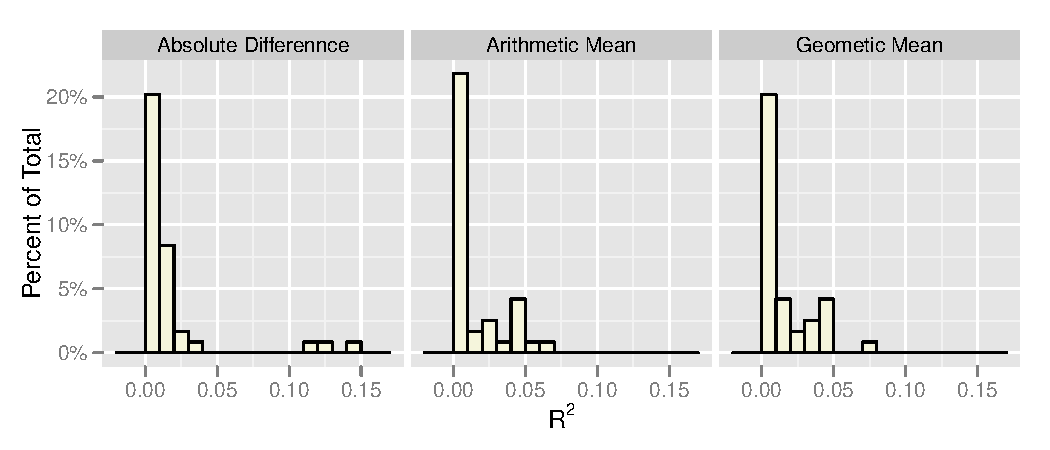
\includegraphics[width=\linewidth]{sali-desc-corr}
}
           
\ctable[cap={}, caption={Plots of predicted versus observed SALI values
  obtained using random forest models, on the Cavalli dataset. Each
  panel corresponds to the use of a different descriptor aggregation
  function.}, label={fig:rfmodel-cavalli}, botcap, figure]
{c}
{}
{
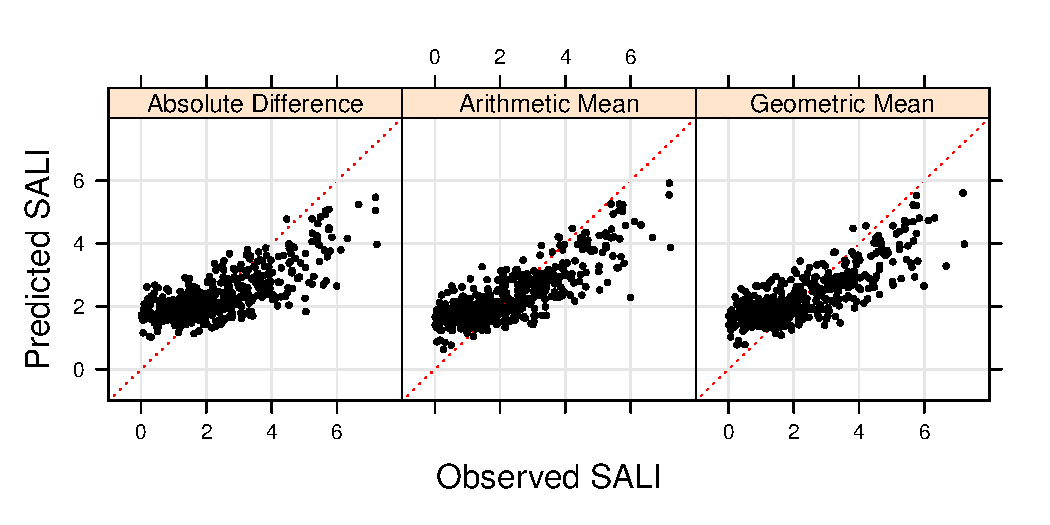
\includegraphics[width=\linewidth]{rfmodels-cavalli}
}

\ctable[cap={}, caption={Predicted versus observed SALI values,
  obtained from random forest models for the three ChEMBL datasets. The
 three plots correspond to the two different aggregation functions
 ($f_{\textrm{diff}}$ and $f_{\textrm{mean}}$ respectively).},
label={fig:rfmodel-chembl},botcap,figure]
{p{0.5in}c}
{}
{
\imagetop{\textbf{Costanzo}} & \imagetop{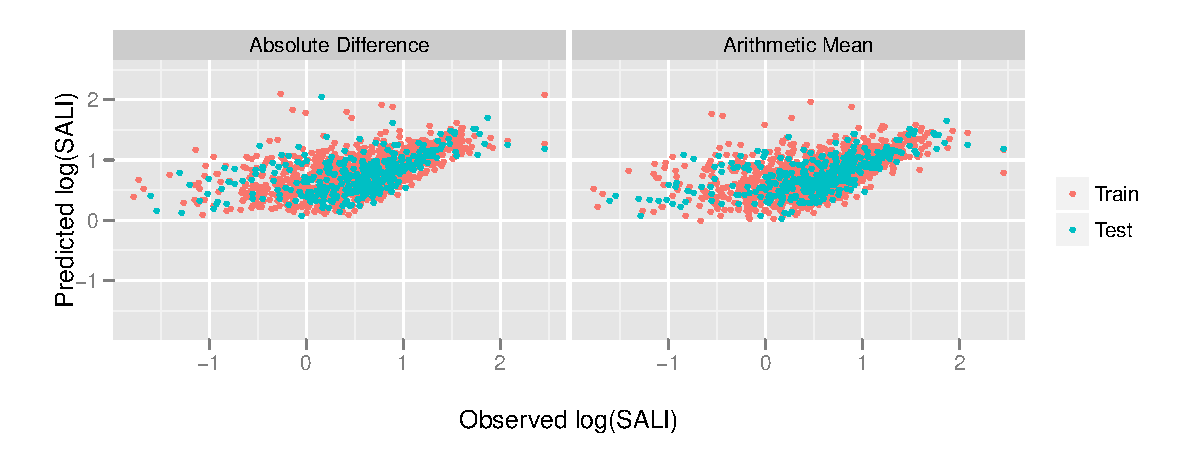
\includegraphics[width=0.9\linewidth]{rfmodels-costanzo}}\NN
\imagetop{\textbf{Kalla}}  & \imagetop{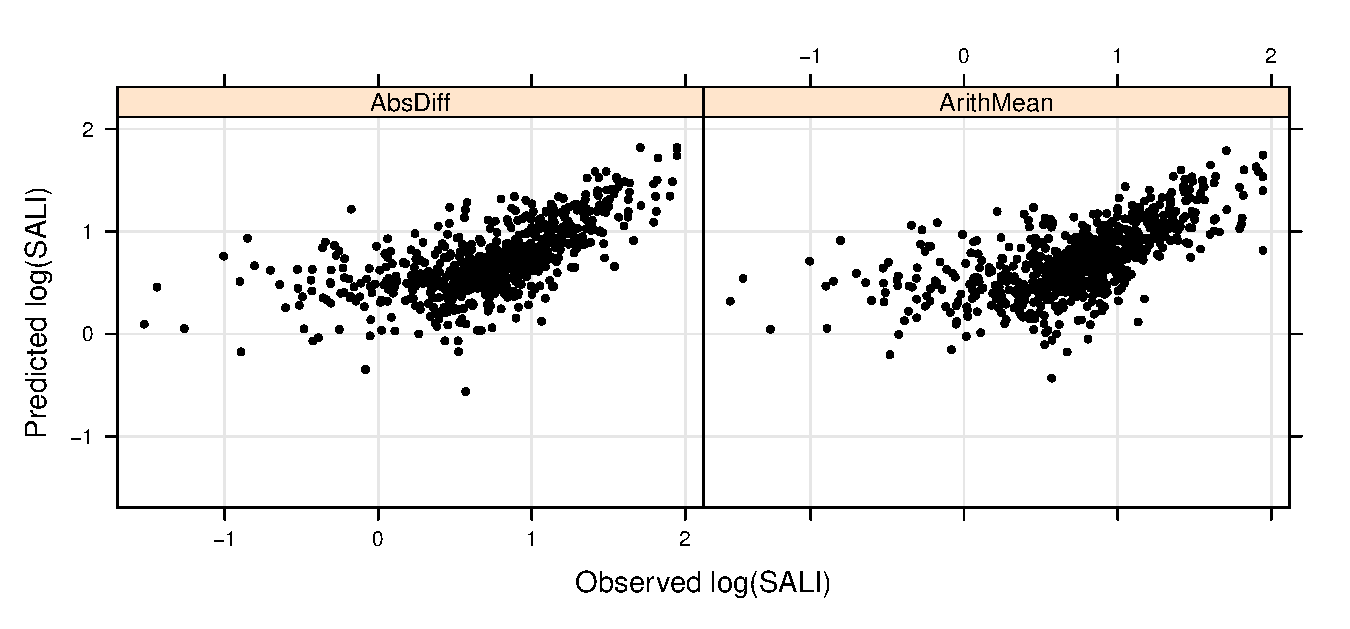
\includegraphics[width=0.9\linewidth]{rfmodels-kalla}} \NN
\imagetop{\textbf{Dai}} &
\imagetop{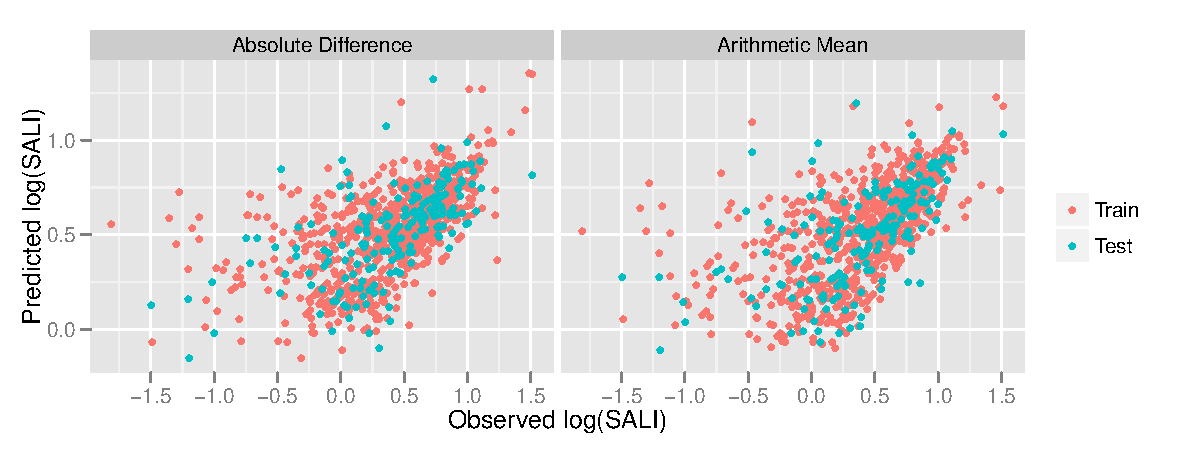
\includegraphics[width=0.9\linewidth]{rfmodels-dai}}   
}


\ctable[cap={}, caption={Results of random forest models developed
  using the Costanzo dataset. The left plot shows the predicted versus
  observed plot for the model using the original $\mathrm{IC_{50}}$ values, and
  the right hand plot shows the predicted versus observed log(SALI)
  values.}, label={fig:costanzo-pred}, figure, botcap]
{c}
{}
{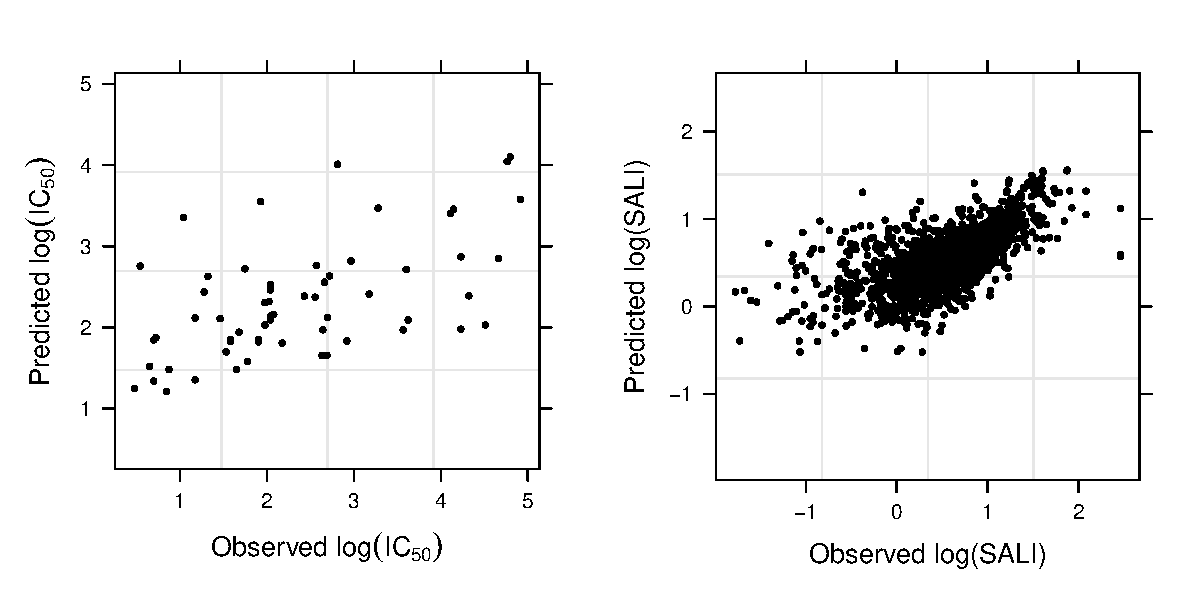
\includegraphics[width=\linewidth]{pred305283}}

\ctable[cap={}, caption={Results of random forest models developed
  using the Kalla dataset. The left plot shows the predicted versus
  observed plot for the model using the original $K_i$ values, and
  the right hand plot shows the predicted versus observed log(SALI)
  values.}, label={fig:kalla-pred}, figure, botcap]
{c}
{}
{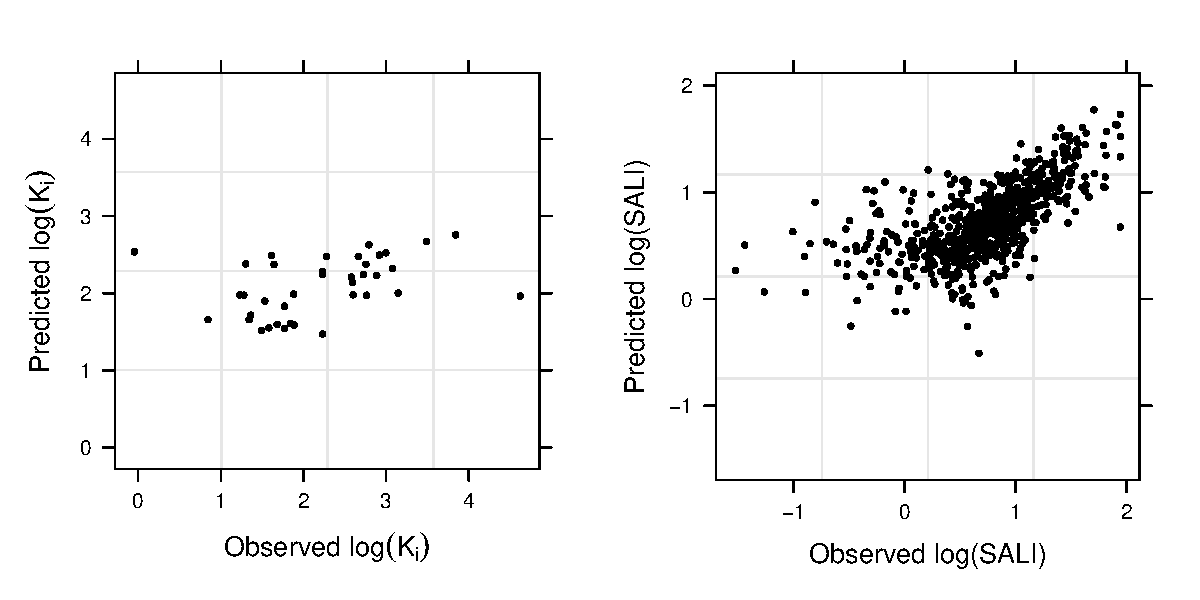
\includegraphics[width=\linewidth]{pred364155}}   


\ctable[cap={}, caption={Results of random forest models developed
  using the Dai dataset. The left plot shows the predicted versus
  observed plot for the model using the original $K_i$ values, and
  the right hand plot shows the predicted versus observed log(SALI)
  values.}, label={fig:dai-pred}, figure, botcap]
{c}
{}
{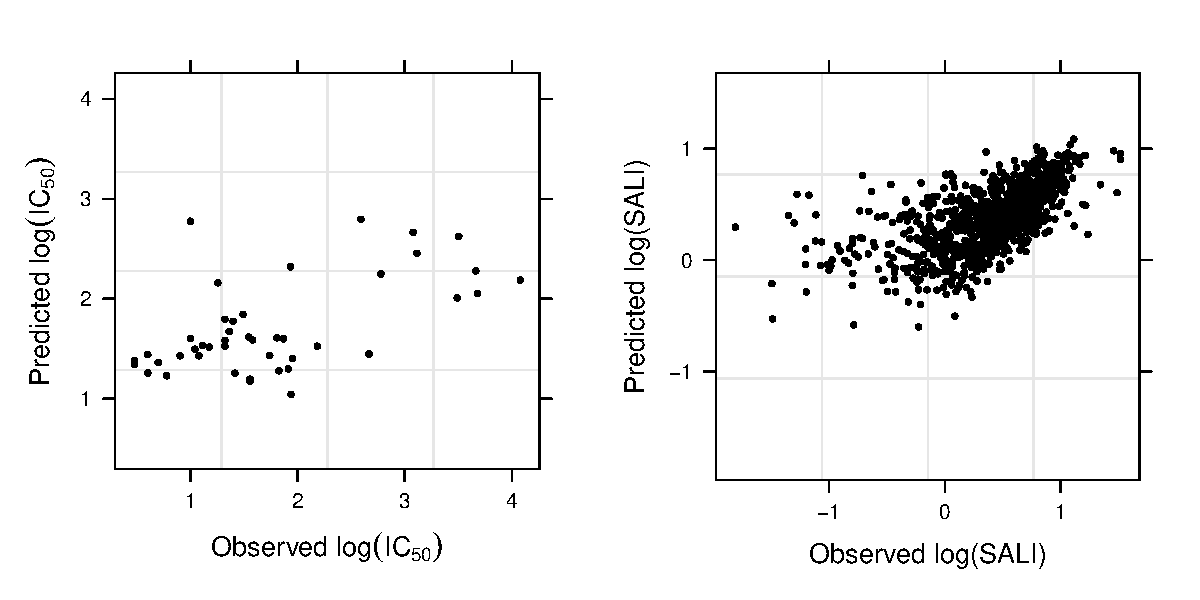
\includegraphics[width=\linewidth]{pred429056}}

 
\ctable[cap={}, caption={Detailed analysis of SALI predictions for the
  Kalla dataset. \textbf{A} - a plot of predicted versus observed
  log(SALI) values for the training set and the hold out
  set. \textbf{B} - a summary of the training set, where we plot the
  structural difference versus the
  logarithm of the ratio of the activities for each pair of molecules
  in the prediction set. Points are shaded by their absolute
residual. \textbf{C} - a box plot summarizing the distribution of  
residuals associated with predictions from each of the hold out molecules.},
label={fig:tset-pset-kalla}, figure, botcap]
{c}
{}
{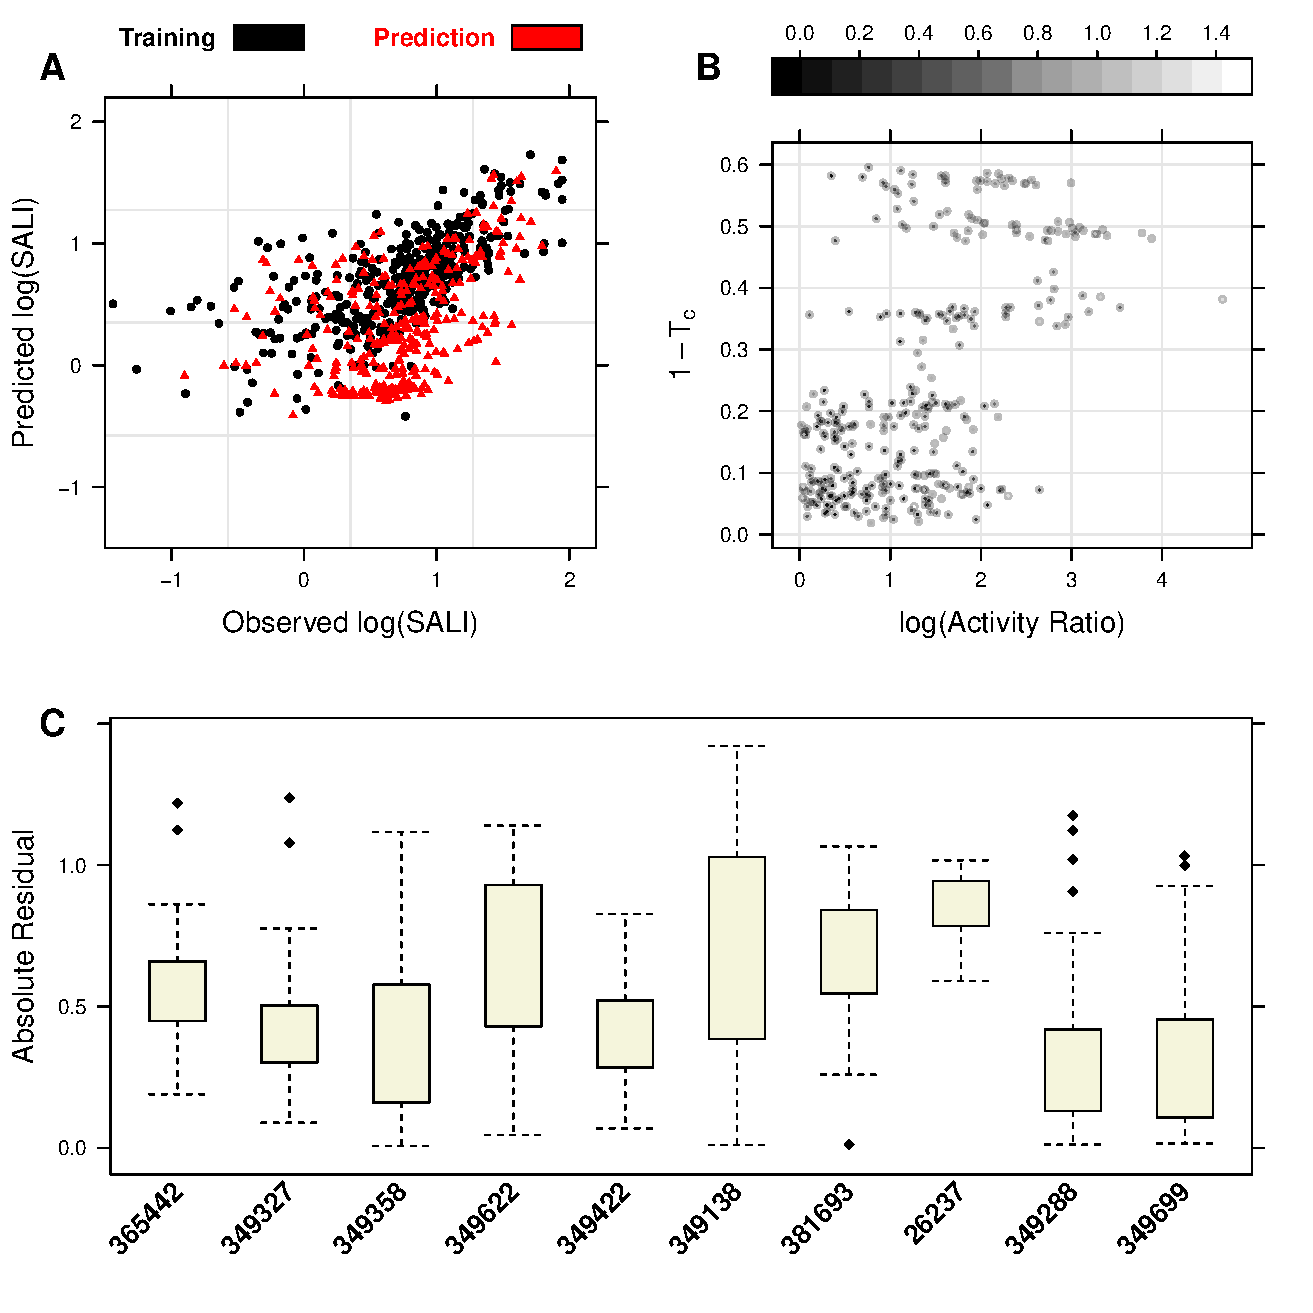
\includegraphics[width=\linewidth]{tset-pset-kalla}}      

\ctable[cap={}, caption={The hold out molecules for the Kalla dataset
  and training set members with which the hold outs exhibit predicted
  activity cliffs. Bold numbers are ChEMBL MOLREGNO values and numbers
  in parentheses are the absolute prediction
  residual in log(SALI) units.}, figure, botcap,
label={fig:kalla-comparison}]    
{c}
{}
{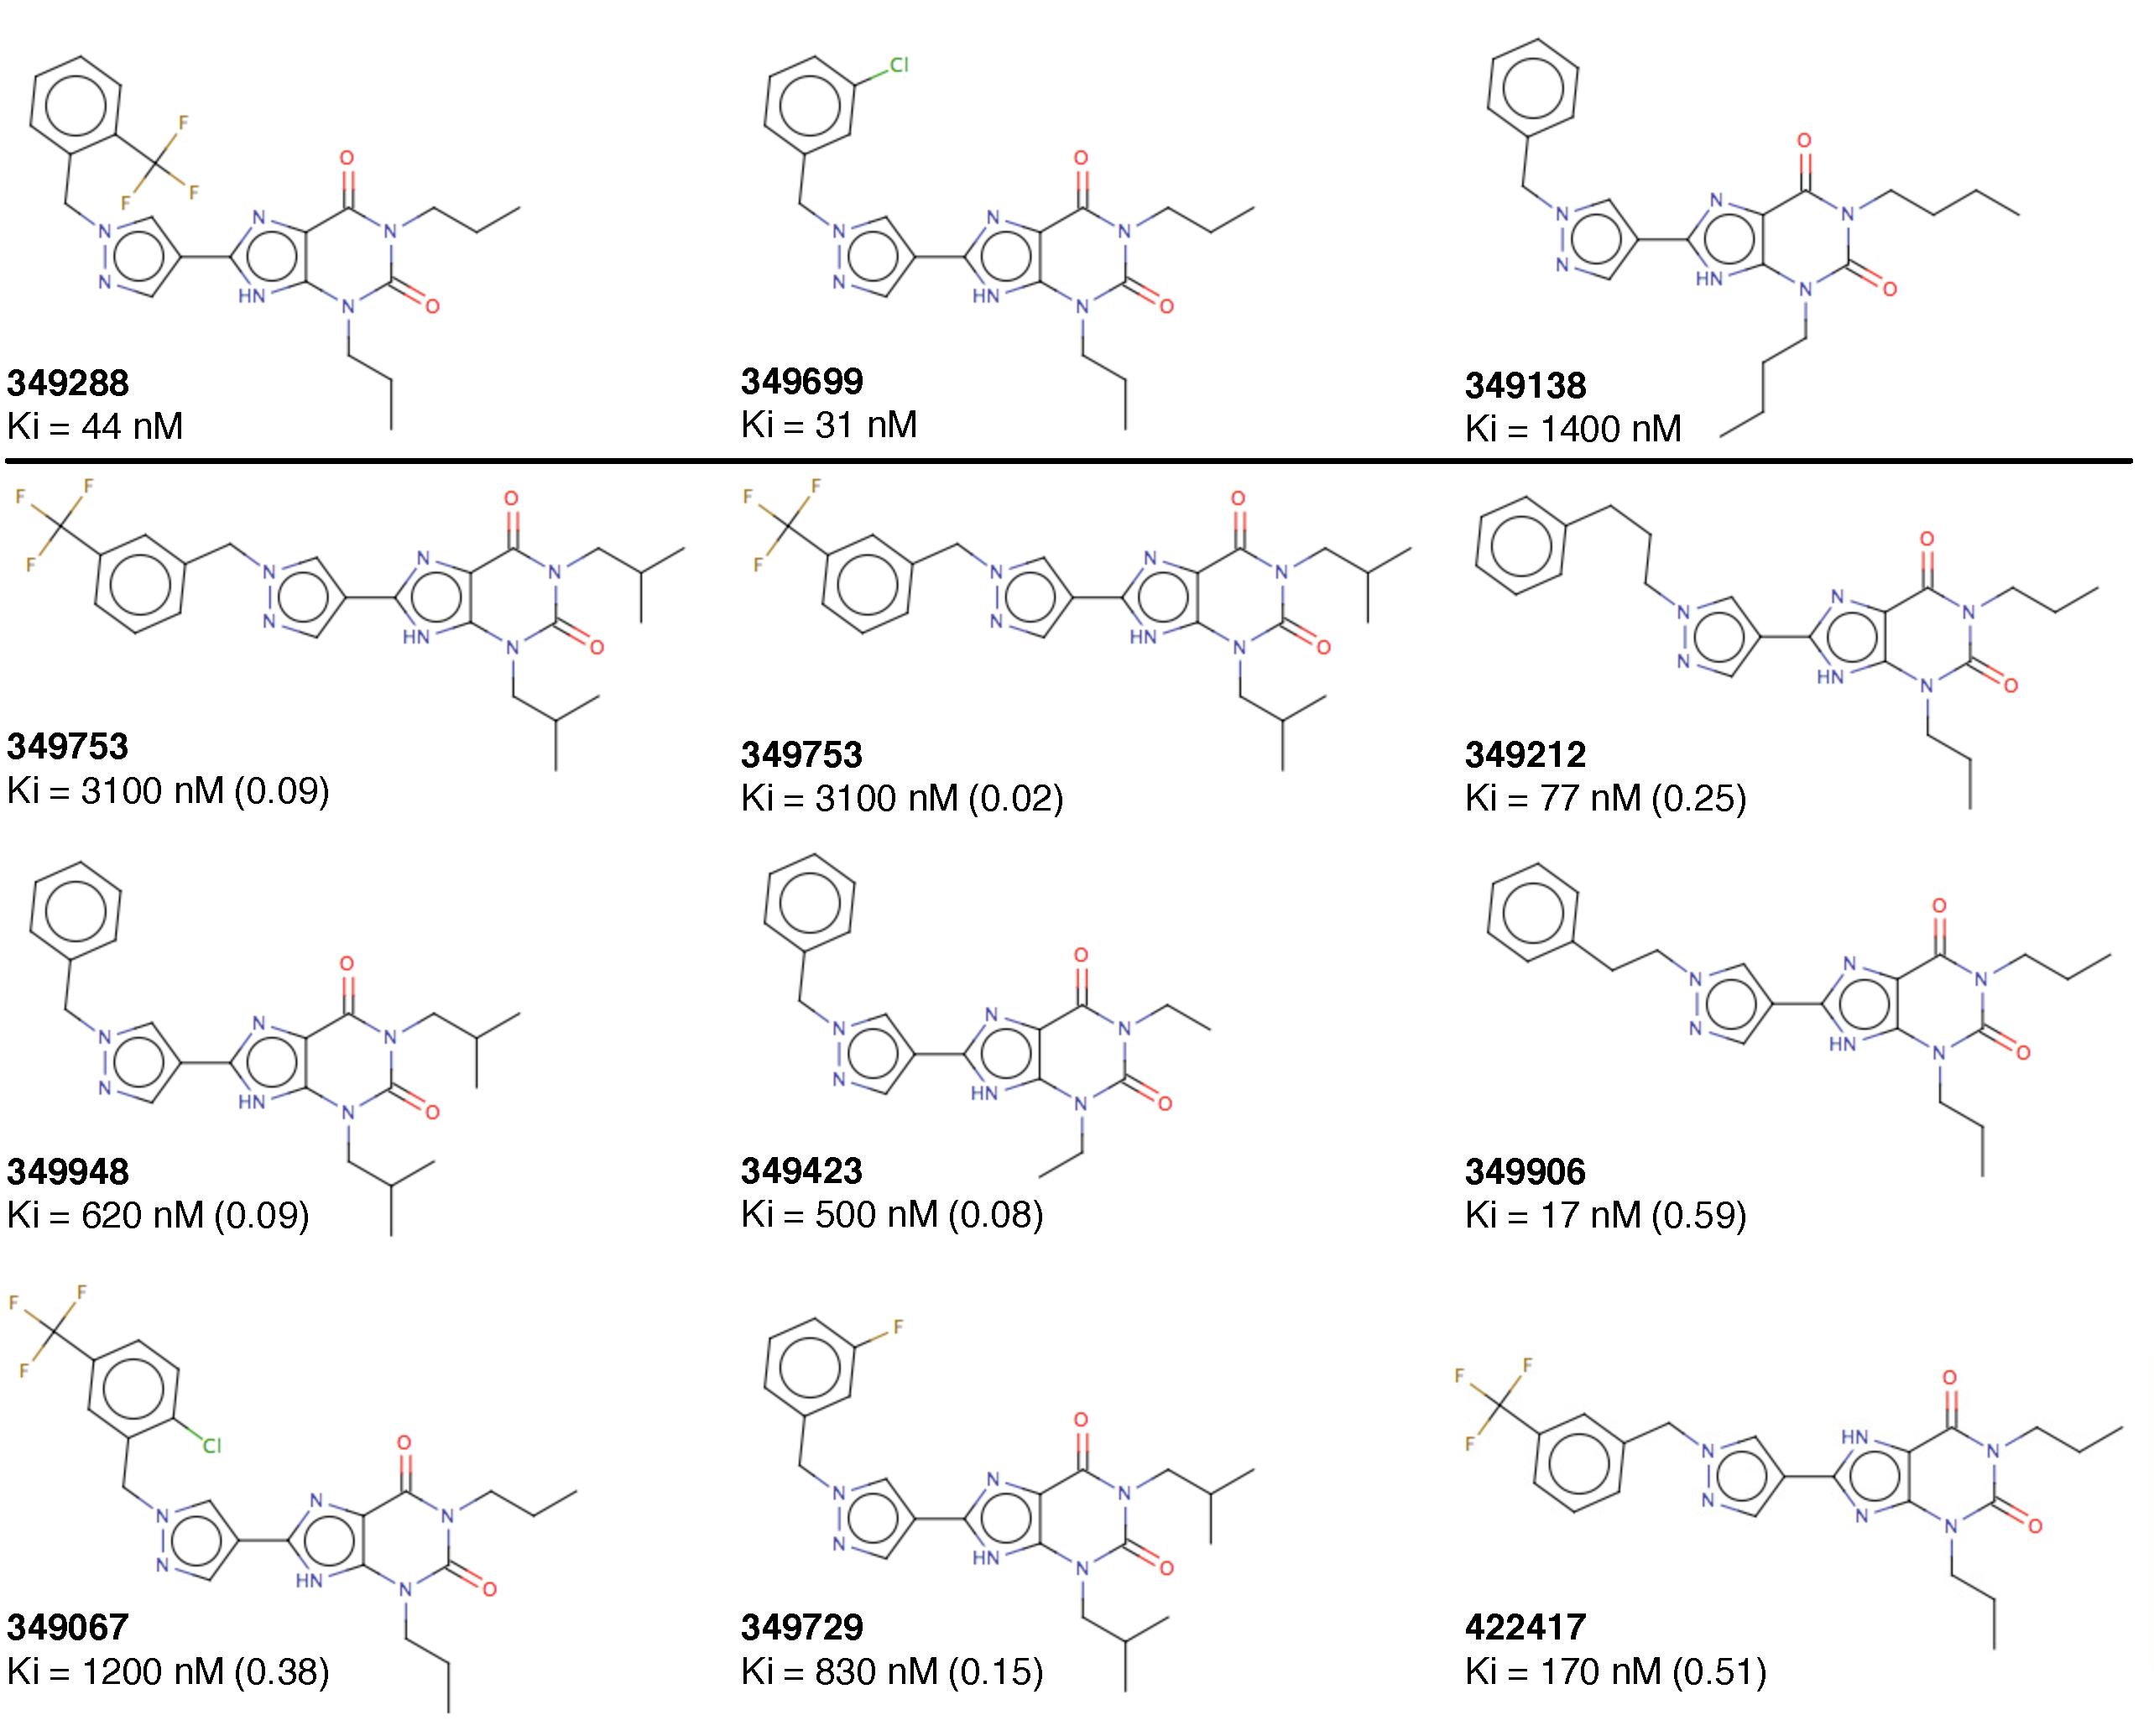
\includegraphics[width=\linewidth]{kalla-comparison}}

\ctable[cap={}, caption={Detailed analysis of SALI predictions for the
  Dai dataset. \textbf{A} - a plot of predicted versus observed
  log(SALI) values for the training set and the hold out
  set. \textbf{B} - a summary of the training set, where we plot the
  structural difference versus the logarithm of the ratio of the
  activities for each pair of molecules
  in the prediction set. Points are shaded by their absolute
  residual. \textbf{C} - a box plot summarizing the distribution of  
  residuals associated with predictions from each of the hold out
  molecules.}, figure, botcap,
label={fig:tset-pset-dai}]    
{c}
{}
{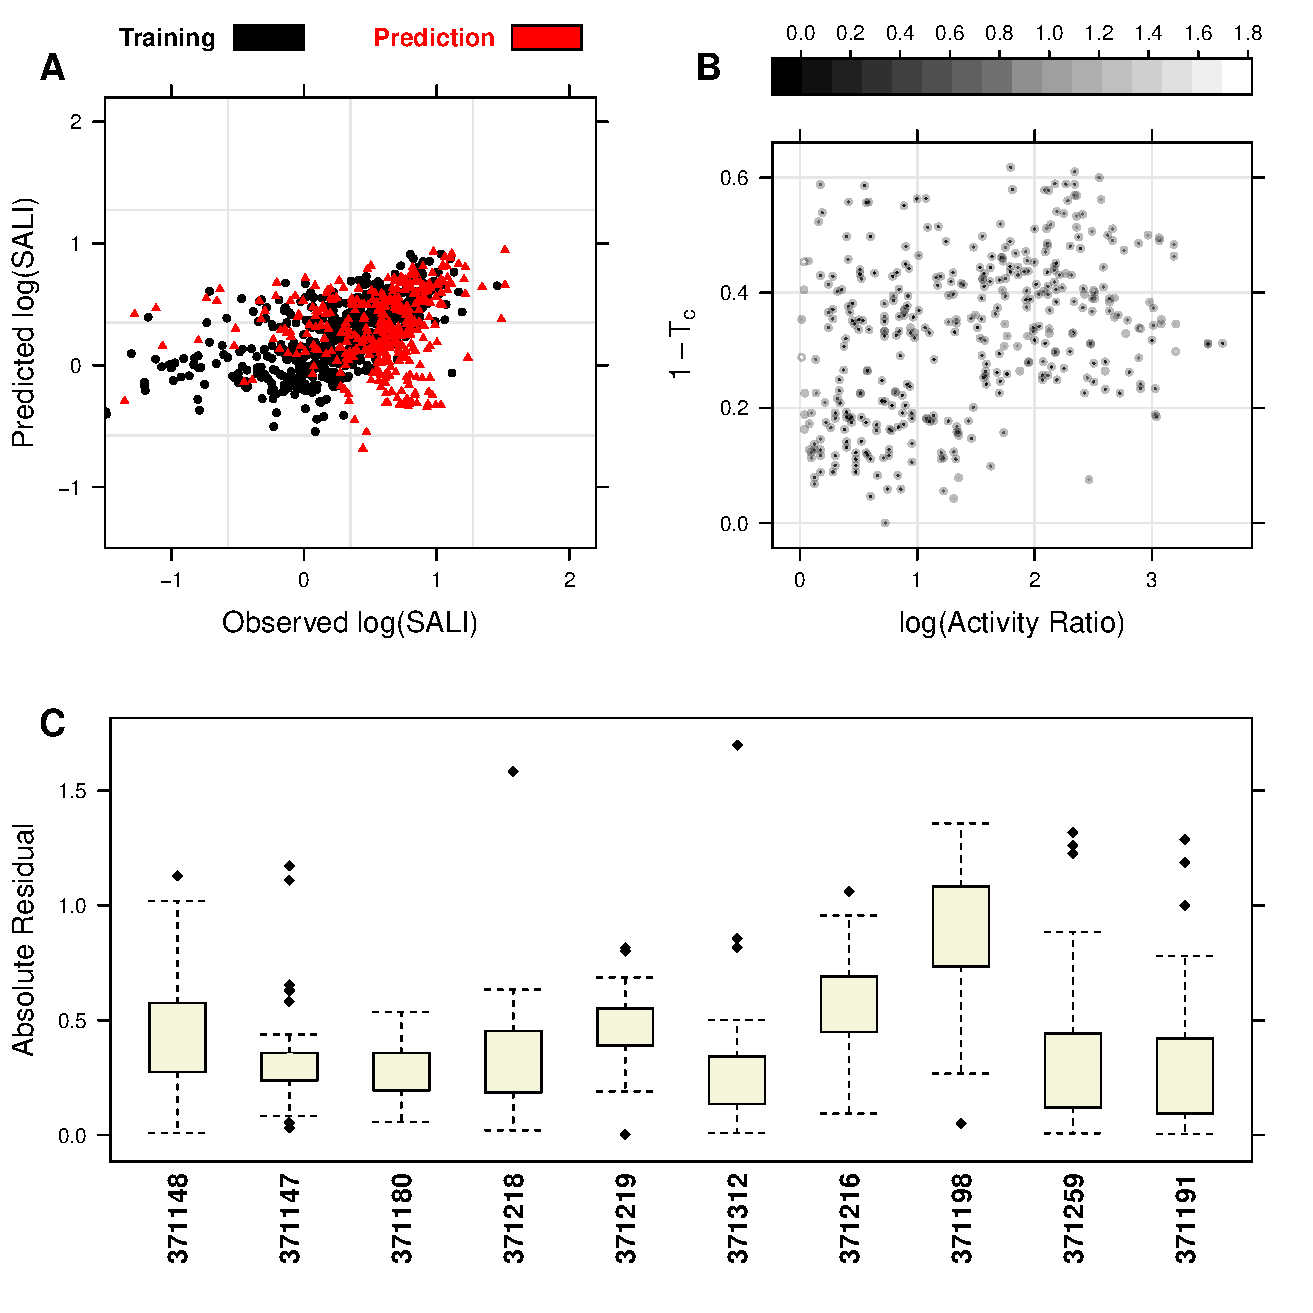
\includegraphics[width=\linewidth]{tset-pset-dai}}

\ctable[cap={}, caption={The hold out molecules for the Dai dataset
  and training set members with which the hold outs exhibit predicted
  activity cliffs. Bold numbers are ChEMBL MOLREGNO values and numbers
  in parentheses are the absolute prediction
  residual in log(SALI) units.}, figure, botcap,
label={fig:dai-comparison}]    
{c}
{}  
{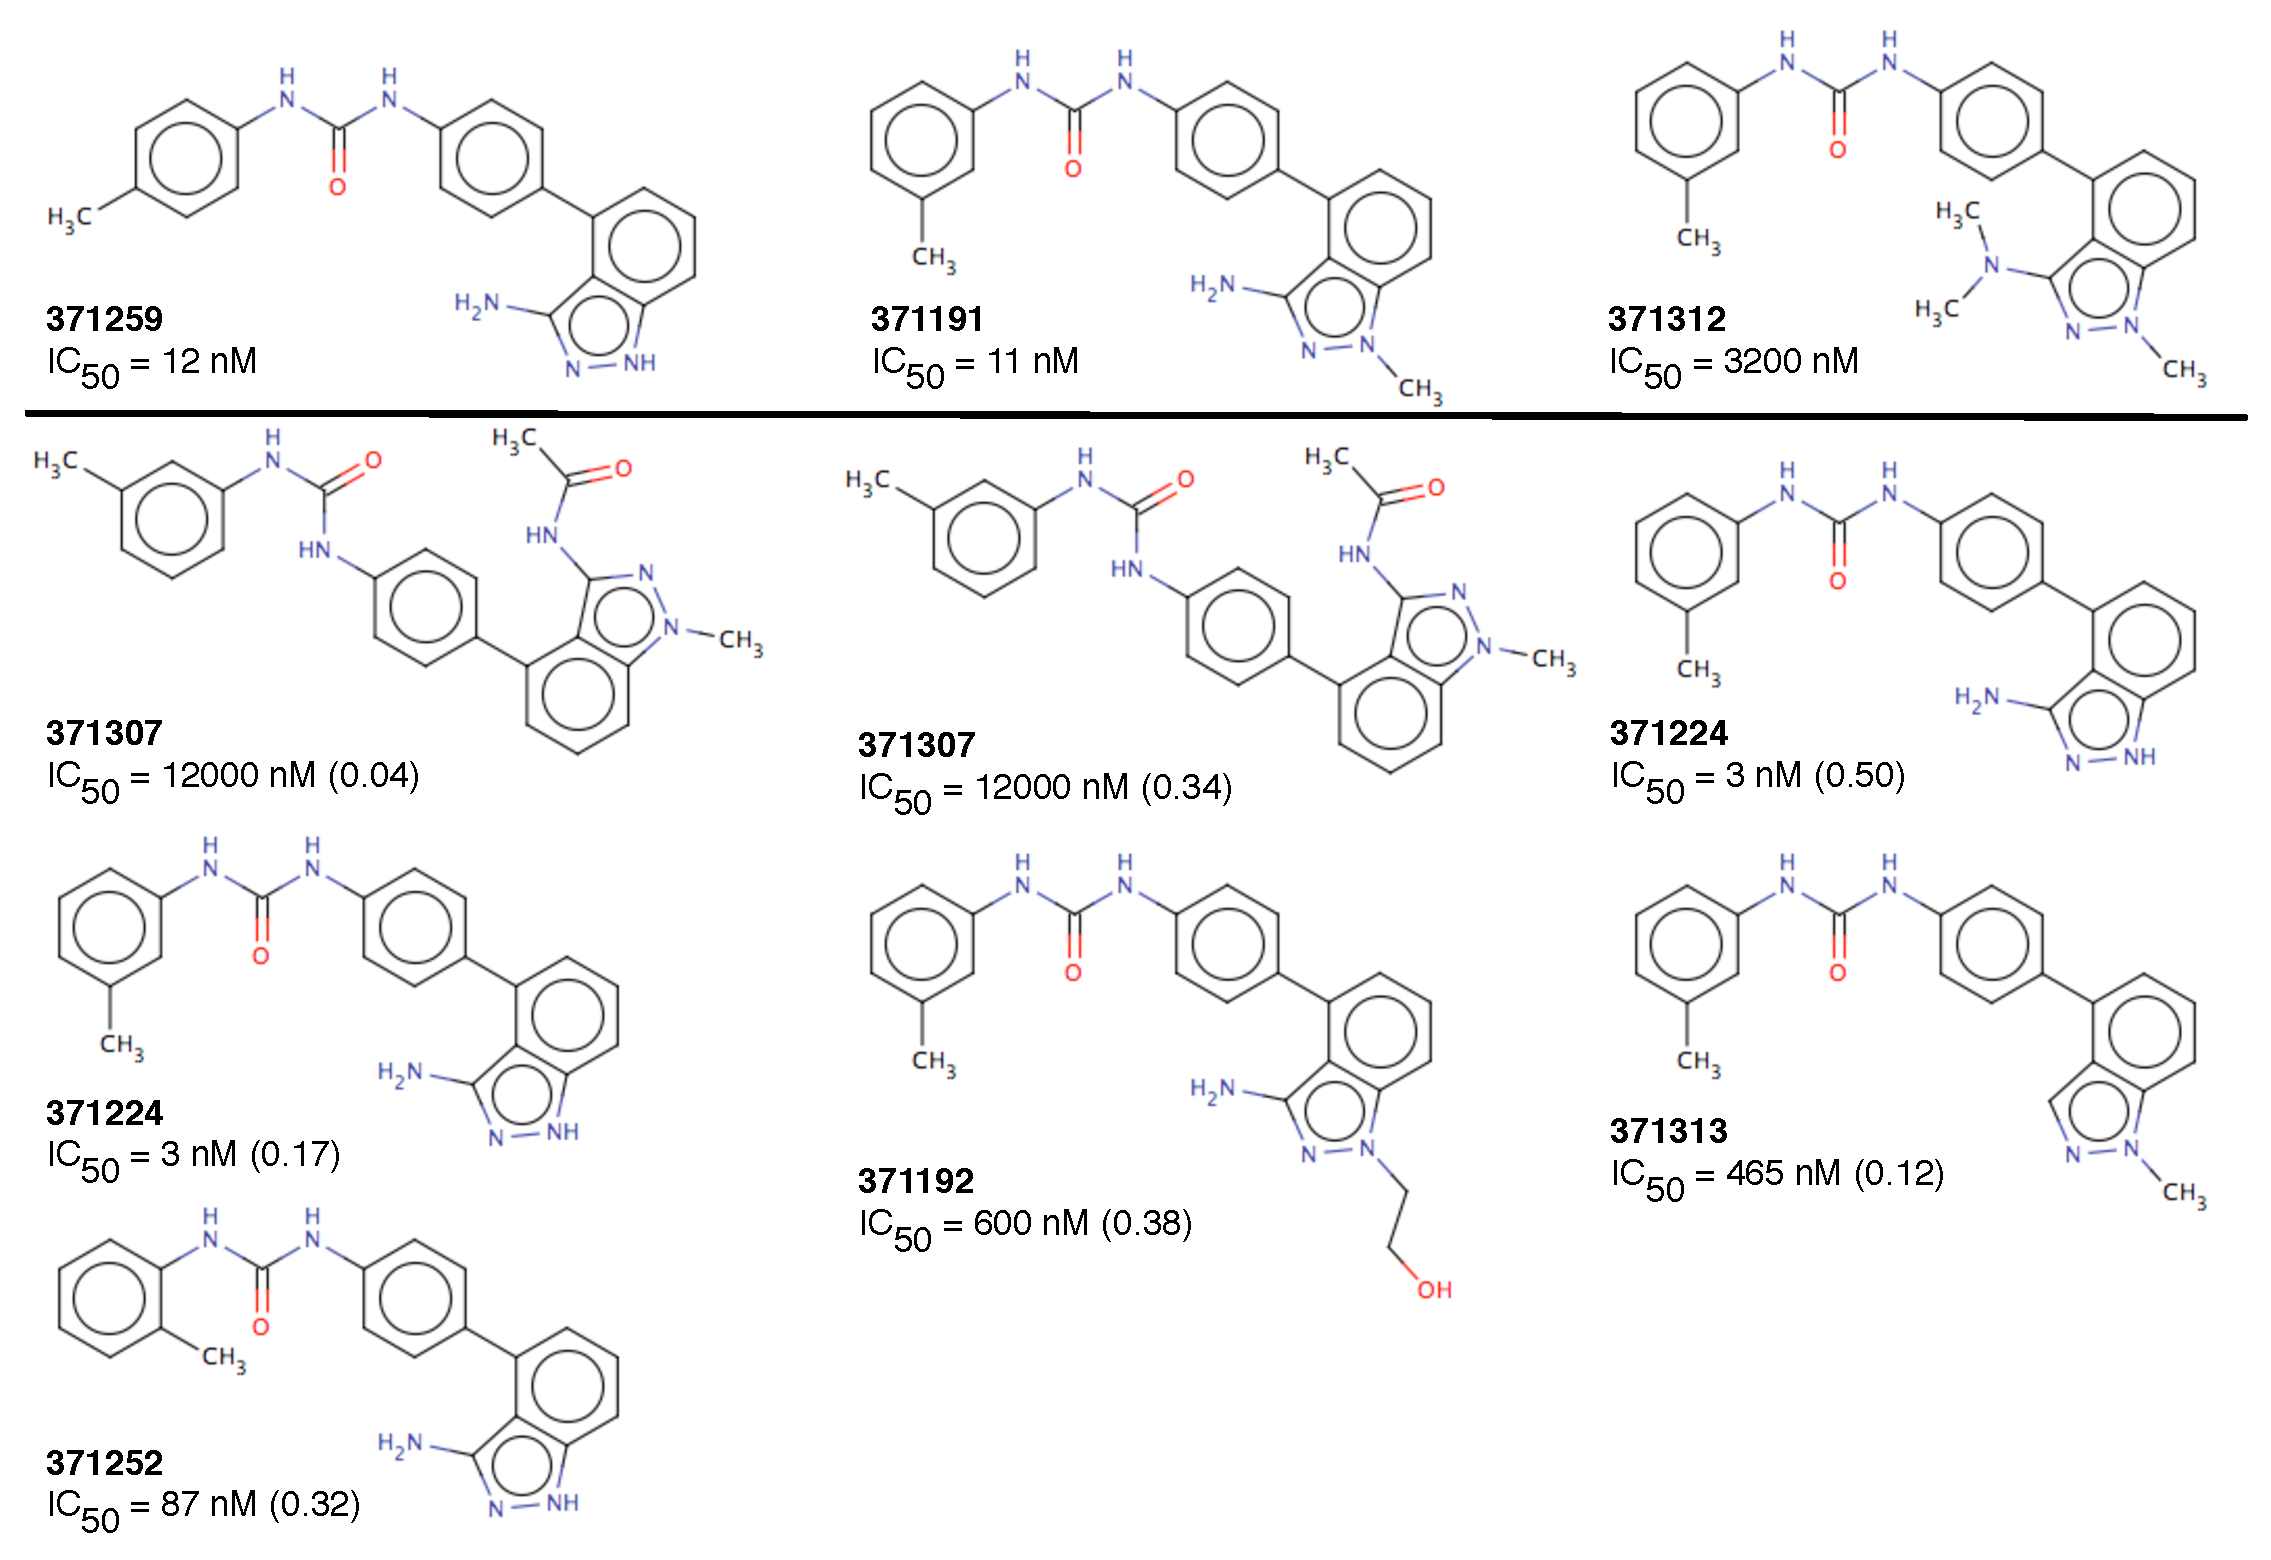
\includegraphics[width=\linewidth]{dai-comparison}}  

\ctable[cap={}, caption={Distribution of log(SALI) values for the
  three ChEMBL datasets.}, figure, botcap,
label={fig:logsalidist}]    
{c}
{}  
{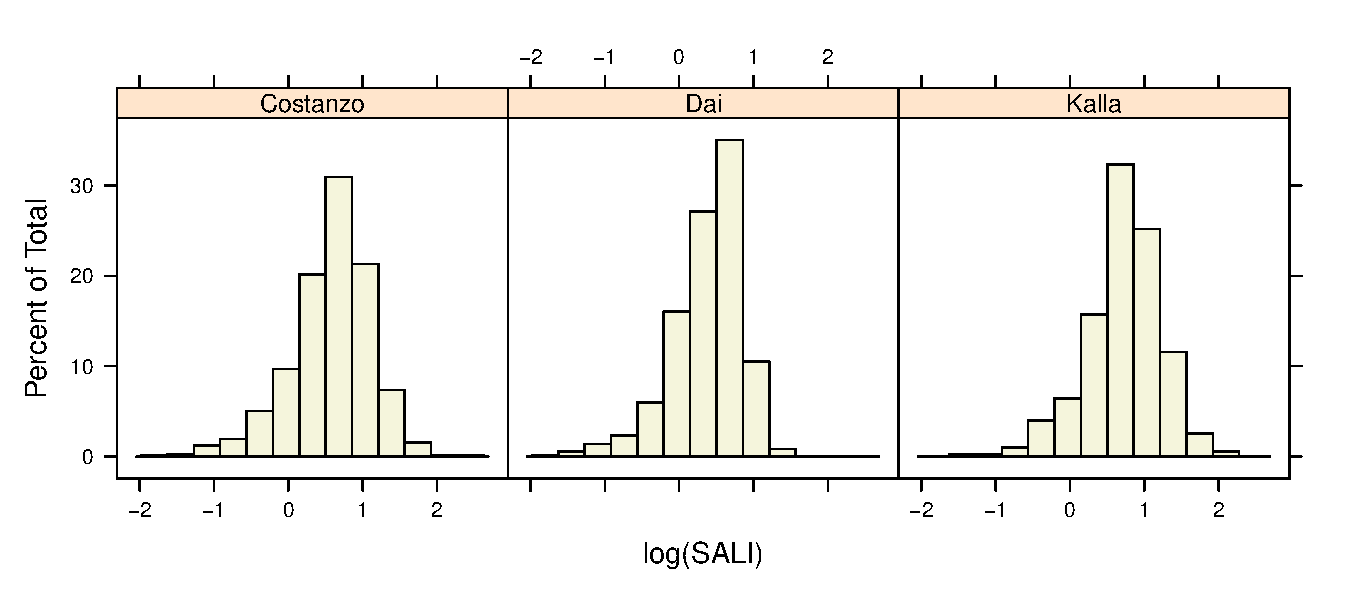
\includegraphics[width=\linewidth]{logsalidist}}  

\end{document}
  
    
     
